\documentclass[kappa, margin=1cm, fontscale=0.28]{baposter}

\usepackage{relsize}	         % For \smaller
\usepackage{url}			         % For \url
\usepackage{epstopdf}	         % Included EPS files automatically converted to PDF to include with pdflatex
\usepackage{multicol}          % Multi Columns
\usepackage{enumitem}          % List Customization
\usepackage{amsmath,amssymb}   % Math
\usepackage{natbib}
\usepackage{graphicx}          % Graphic Display
\usepackage{pgf}               % Graphics and special plotting
\usepackage{tikz}              % draw
\usepackage{xcolor}            % colurs
\usepackage{hyperref}          % linx

% \definecolor{umblue}{rgb}{0.03, 0.15, 0.30}
\definecolor{umblue}{HTML}{00274C}
% \definecolor{ummaize}{rgb}{0.90, 0.85, 0.40}
\definecolor{ummaize}{HTML}{FFCB05}

%%%%%%%%%%%%%%%%%%%%%%%%%%%%%%%%%%%%%%%%%%%%%%%%%%%%%%%%%%%%%%%%%%%%%%%%%%%%%%%%%%%%%
%%% Utility functions %%%%%%%%%%%%%%%%%%%%%%%%%%%%%%%%%%%%%%%%%%%%%%%%%%%%%%%%%%%%%%%
%%%%%%%%%%%%%%%%%%%%%%%%%%%%%%%%%%%%%%%%%%%%%%%%%%%%%%%%%%%%%%%%%%%%%%%%%%%%%%%%%%%%%

%%%%%%%%%%%%%%%%%%%%%%%%%%%%%%%%%%%%%%%%%%%%%%%%%%%%%%%%%%%%%%%%%%%%%%%%%%%%%%%%%%%%%
%%% Save space in lists. Use this after the opening of the list %%%%%%%%%%%%%%%%%%%%%
%%%%%%%%%%%%%%%%%%%%%%%%%%%%%%%%%%%%%%%%%%%%%%%%%%%%%%%%%%%%%%%%%%%%%%%%%%%%%%%%%%%%%
\renewcommand{\vec}[1]{\bm{#1}}
\newcommand{\vnabla}{\vec{\nabla}}

\renewcommand{\d}[1]{\text{d} #1}
\newcommand{\dxx}{\,\text{d}\vec{x}}
\newcommand{\dx}{\,\text{d}x}

\newcommand{\diff}[2]{\frac{\text{d}#1}{\text{d}#2}}
\newcommand{\idiff}[2]{\text{d}#1 / \text{d}#2}
\newcommand{\pdiff}[2]{\frac{\partial #1}{\partial #2}}
\newcommand{\pdifff}[2]{\frac{\partial^2 #1}{\partial #2^2}}
\newcommand{\ipdiff}[2]{\partial #1 / \partial #2}
\newcommand{\vdiff}[2]{\frac{\delta #1}{\delta #2}}
\newcommand{\ivdiff}[2]{\delta #1 / \delta #2}

%%%%%%%%%%%%%%%%%%%%%%%%%%%%%%%%%%%%%%%%%%%%%%%%%%%%%%%%%%%%%%%%%%%%%%%%%%%%%%%%%%%%
%%% Document Start %%%%%%%%%%%%%%%%%%%%%%%%%%%%%%%%%%%%%%%%%%%%%%%%%%%%%%%%%%%%%%%%%
%%%%%%%%%%%%%%%%%%%%%%%%%%%%%%%%%%%%%%%%%%%%%%%%%%%%%%%%%%%%%%%%%%%%%%%%%%%%%%%%%%%%

\begin{document}
\typeout{Poster rendering started}

%%%%%%%%%%%%%%%%%%%%%%%%%%%%%%%%%%%%%%%%%%%%%%%%%%%%%%%%%%%%%%%%%%%%%%%%%%%%%%%%%%%%
%%% General Poster Settings %%%%%%%%%%%%%%%%%%%%%%%%%%%%%%%%%%%%%%%%%%%%%%%%%%%%%%%%
%%%%%% Eye Catcher, Title, Authors and University Images %%%%%%%%%%%%%%%%%%%%%%%%%%%
%%%%%%%%%%%%%%%%%%%%%%%%%%%%%%%%%%%%%%%%%%%%%%%%%%%%%%%%%%%%%%%%%%%%%%%%%%%%%%%%%%%%
\begin{poster}{
    columns=4,
    grid=false,
    borderColor=umblue,
    headerColorOne=umblue,
    headerColorTwo=umblue,
    headerFontColor=ummaize,
    headerheight=13em,
    boxColorOne=white,
    boxColorTwo=umblue,
    linewidth=1.5pt,
    boxpadding=0.55em,
    headershape=rectangle,
    headerfont=\Large\textsf,
    textborder=faded,
    background=plain,
    bgColorOne=white,
    bgColorTwo=umblue,
    headerborder=closed,
    boxshade=plain,
    headershade=plain,
    eyecatcher=false
}
%%%%%%%%%%%%%%%%%%%%%%%%%%%%%%%%%%%%%%%%%%%%%%%%%%%%%%%%%%%%%%%%%%%%%%%%%%%%%%%%%%%%
%%% Eye Catcher %%%%%%%%%%%%%%%%%%%%%%%%%%%%%%%%%%%%%%%%%%%%%%%%%%%%%%%%%%%%%%%%%%%%
%%%%%%%%%%%%%%%%%%%%%%%%%%%%%%%%%%%%%%%%%%%%%%%%%%%%%%%%%%%%%%%%%%%%%%%%%%%%%%%%%%%%
{
}
%%%%%%%%%%%%%%%%%%%%%%%%%%%%%%%%%%%%%%%%%%%%%%%%%%%%%%%%%%%%%%%%%%%%%%%%%%%%%%%%%%%%
%%% Title %%%%%%%%%%%%%%%%%%%%%%%%%%%%%%%%%%%%%%%%%%%%%%%%%%%%%%%%%%%%%%%%%%%%%%%%%%
%%%%%%%%%%%%%%%%%%%%%%%%%%%%%%%%%%%%%%%%%%%%%%%%%%%%%%%%%%%%%%%%%%%%%%%%%%%%%%%%%%%%
{Assessing the Ecology of the Flint River, \\ Above and Below a Century-Old Dam}
%%%%%%%%%%%%%%%%%%%%%%%%%%%%%%%%%%%%%%%%%%%%%%%%%%%%%%%%%%%%%%%%%%%%%%%%%%%%%%%%%%%%
%%% Authors %%%%%%%%%%%%%%%%%%%%%%%%%%%%%%%%%%%%%%%%%%%%%%%%%%%%%%%%%%%%%%%%%%%%%%%%
%%%%%%%%%%%%%%%%%%%%%%%%%%%%%%%%%%%%%%%%%%%%%%%%%%%%%%%%%%%%%%%%%%%%%%%%%%%%%%%%%%%%
{
  \vspace{0mm}
  \text{Chloe Summers} : \textit{\color{violet}{summersj@umich.edu}}, 
  \text{Arianna Elkins} : \textit{\color{violet}{arelkins@umich.edu}}, \\
  \text{Cason Konzer} : \textit{\color{violet}{casonk@umich.edu}}, 
  \text{Heather Dawson} : \textit{\color{violet}{hdawson@umich.edu}} 
  
  \hspace{1mm} {\color{umblue}$\downharpoonright$} repository : 
  \textit{\color{violet}{https://github.com/casonk/Flint\_River\_Ecology}}
  \hspace{1mm} {\color{umblue}$\downharpoonright$} website : 
  \textit{\color{violet}{https://flintriverecostudy.com}}
}
%%%%%%%%%%%%%%%%%%%%%%%%%%%%%%%%%%%%%%%%%%%%%%%%%%%%%%%%%%%%%%%%%%%%%%%%%%%%%%%%%%%%
%%% Logo %%%%%%%%%%%%%%%%%%%%%%%%%%%%%%%%%%%%%%%%%%%%%%%%%%%%%%%%%%%%%%%%%%%%%%%%%%%
%%%%%%%%%%%%%%%%%%%%%%%%%%%%%%%%%%%%%%%%%%%%%%%%%%%%%%%%%%%%%%%%%%%%%%%%%%%%%%%%%%%%
{
  \begin{minipage}{9.0em}
    
\includegraphics[height=9em]{Img/Ecology_Study.png}
  \end{minipage}
  \begin{minipage}{9.0em}
    
\includegraphics[height=9em]{Img/University_of_Michigan_Flint.png}
  \end{minipage}
}
%%%%%%%%%%%%%%%%%%%%%%%%%%%%%%%%%%%%%%%%%%%%%%%%%%%%%%%%%%%%%%%%%%%%%%%%%%%%%%%%%%%%
%%% Where is Flint? %%%%%%%%%%%%%%%%%%%%%%%%%%%%%%%%%%%%%%%%%%%%%%%%%%%%%%%%%%%%%%%%
%%%%%%%%%%%%%%%%%%%%%%%%%%%%%%%%%%%%%%%%%%%%%%%%%%%%%%%%%%%%%%%%%%%%%%%%%%%%%%%%%%%%
\headerbox{Where is Flint?}{name=box00, column=0, row=0}{
    \begin{center}
      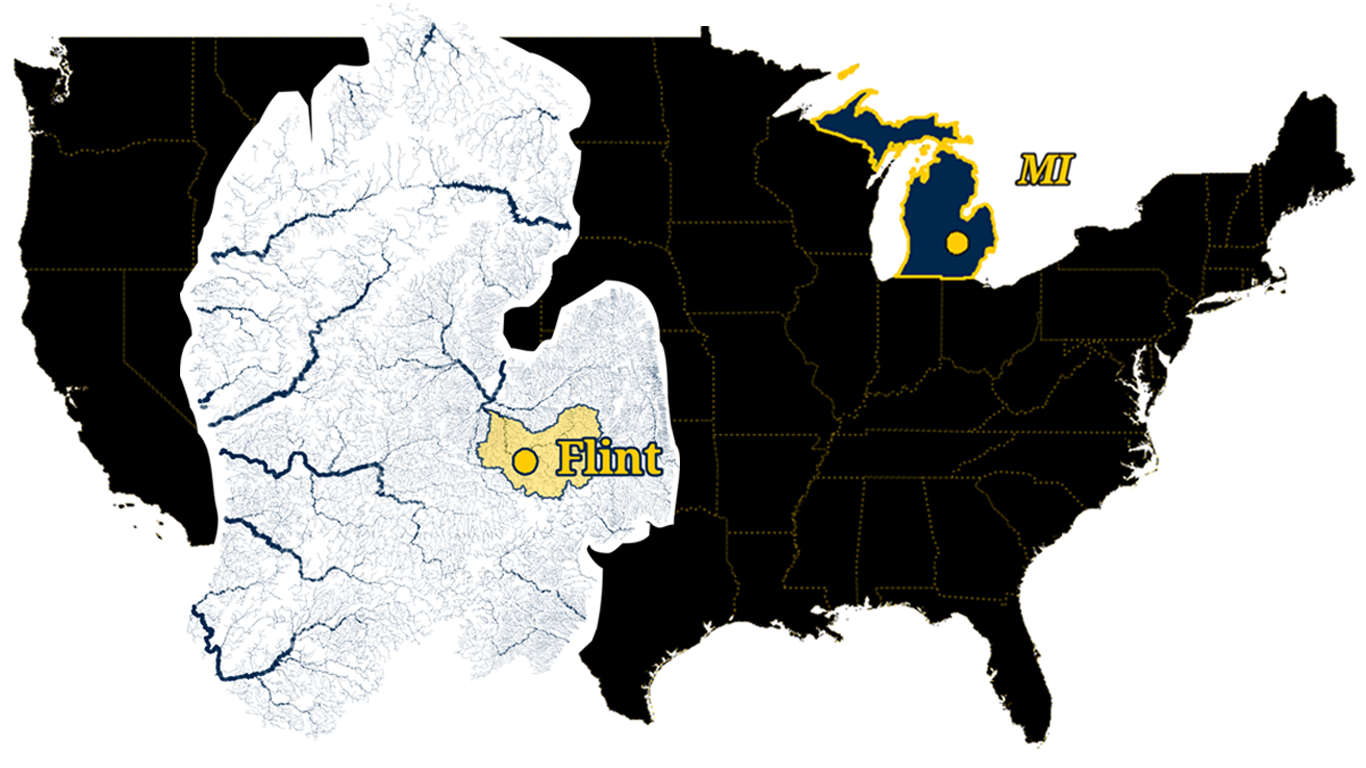
\includegraphics[width=0.95\textwidth]{Img/Combo_Map.png}

    \end{center}
    {\small
    Figure 1. Michigan location in USA and Flint location in MI. 
    }
}
%%%%%%%%%%%%%%%%%%%%%%%%%%%%%%%%%%%%%%%%%%%%%%%%%%%%%%%%%%%%%%%%%%%%%%%%%%%%%%%%%%%%
%%% Introduction %%%%%%%%%%%%%%%%%%%%%%%%%%%%%%%%%%%%%%%%%%%%%%%%%%%%%%%%%%%%%%%%%%%
%%%%%%%%%%%%%%%%%%%%%%%%%%%%%%%%%%%%%%%%%%%%%%%%%%%%%%%%%%%%%%%%%%%%%%%%%%%%%%%%%%%%
\headerbox{Introduction}{name=box01, column=0, row=1, below=box00}{
  \begin{itemize}[leftmargin=11.5pt]
    \normalsize 
    \item The Hamilton Dam is the terminal dam on the 
    Flint River and was constructed in 1920. 
    The dam is in the urban city of Flint, Michigan and prevents fish passage upstream, 
    but many fish migrate from the Great Lakes to this dam during spawning periods.
    \item Upstream reaches of the Hamilton dam consist of a wide riparian zone, 
    whereas downstream is composed mainly of cemented structures.
  \end{itemize}
}
%%%%%%%%%%%%%%%%%%%%%%%%%%%%%%%%%%%%%%%%%%%%%%%%%%%%%%%%%%%%%%%%%%%%%%%%%%%%%%%%%%%%
%%% Hypotheses %%%%%%%%%%%%%%%%%%%%%%%%%%%%%%%%%%%%%%%%%%%%%%%%%%%%%%%%%%%%%%%%%%%%%
%%%%%%%%%%%%%%%%%%%%%%%%%%%%%%%%%%%%%%%%%%%%%%%%%%%%%%%%%%%%%%%%%%%%%%%%%%%%%%%%%%%%
\headerbox{Hypotheses}{name=box02, column=0, row=2, below=box01}{
  \textbf{
  \begin{enumerate}[leftmargin=14pt]
    \normalsize 
    \item Because of influences from Great Lakes fishes, 
    contaminant loads of fishes will be higher downstream than upstream. 
    \item Due to habitat availability, 
    water \\ quality scores based on benthic 
    macroinvertebrate communities will be higher upstream than downstream.
    \item Because many Great Lakes fishes \\ migrate to the dam, 
    fish population \\ diversity indices will be higher
    \\ downstream of this terminal dam than upstream.
  \end{enumerate}
  }
}
%%%%%%%%%%%%%%%%%%%%%%%%%%%%%%%%%%%%%%%%%%%%%%%%%%%%%%%%%%%%%%%%%%%%%%%%%%%%%%%%%%%%
%%% Methods %%%%%%%%%%%%%%%%%%%%%%%%%%%%%%%%%%%%%%%%%%%%%%%%%%%%%%%%%%%%%%%%%%%%%%%%
%%%%%%%%%%%%%%%%%%%%%%%%%%%%%%%%%%%%%%%%%%%%%%%%%%%%%%%%%%%%%%%%%%%%%%%%%%%%%%%%%%%%
\headerbox{Methods}{name=box03, column=0, row=3, above=bottom, below=box02}{
  \begin{itemize}[leftmargin=11.5pt]
    \normalsize 
    \item Fish were obtained from four sites near the Hamilton Dam (Figure 2) 
    using cast nets, \\ gillnets, hoop traps, electrofishing (Figure 3), 
    and hook and line and select fish were \\ preserved for contaminant analysis. 
    \item Benthic macroinvertebrates were sampled \\ upstream and 
    downstream of the dam in the spring and fall and water quality scores were assessed.
    \item Fish species were obtained and  measured, weighed, tagged (Figure 3), 
    and released and diversity indices were compared downstream vs. upstream. 
  \end{itemize}
}
%%%%%%%%%%%%%%%%%%%%%%%%%%%%%%%%%%%%%%%%%%%%%%%%%%%%%%%%%%%%%%%%%%%%%%%%%%%%%%%%%%%%
%%% Methods %%%%%%%%%%%%%%%%%%%%%%%%%%%%%%%%%%%%%%%%%%%%%%%%%%%%%%%%%%%%%%%%%%%%%%%%
%%%%%%%%%%%%%%%%%%%%%%%%%%%%%%%%%%%%%%%%%%%%%%%%%%%%%%%%%%%%%%%%%%%%%%%%%%%%%%%%%%%%
\headerbox{Methods}{name=box10, column=1, row=0}{
  \begin{center}
    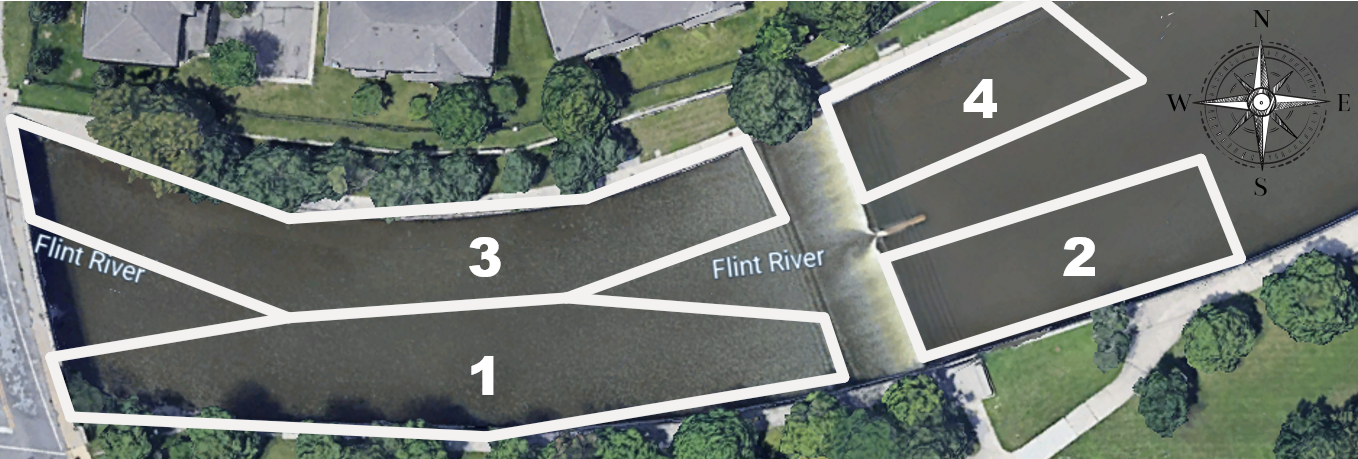
\includegraphics[width=0.99\textwidth]{Img/Site_Map.png} \\

  \end{center}
  {\small
  Figure 2. Study site map for the \\ Flint River Ecology Study.
  } \\

  \textbf{\noindent
  Collect data on the ecology and health of the Flint River above and below the Hamilton Dam 
  before the dam removal and the restoration of the Flint River to gain an understanding of 
  the present ecosystem and provide a baseline for \\ measures of restoration outcomes.
  }

  \begin{center}
    \includegraphics[width=0.99\textwidth]{Img/Methods.png} \\

  \end{center}
  {\small
  Figure 3. Sampling Methods. \\
  Top-Left:Hoop Trap, 
  Top-Right:Electrofishing, \\
  Bottom-Left:Tagging, 
  Bottom-Right:Cast Net.
  }
}
%%%%%%%%%%%%%%%%%%%%%%%%%%%%%%%%%%%%%%%%%%%%%%%%%%%%%%%%%%%%%%%%%%%%%%%%%%%%%%%%%%%%
%%% Contaminant Analysis %%%%%%%%%%%%%%%%%%%%%%%%%%%%%%%%%%%%%%%%%%%%%%%%%%%%%%%%%%%
%%%%%%%%%%%%%%%%%%%%%%%%%%%%%%%%%%%%%%%%%%%%%%%%%%%%%%%%%%%%%%%%%%%%%%%%%%%%%%%%%%%%
\headerbox{Contaminant Analysis}{name=box11, column=1, row=1, below=box10}{
  \begin{center}
    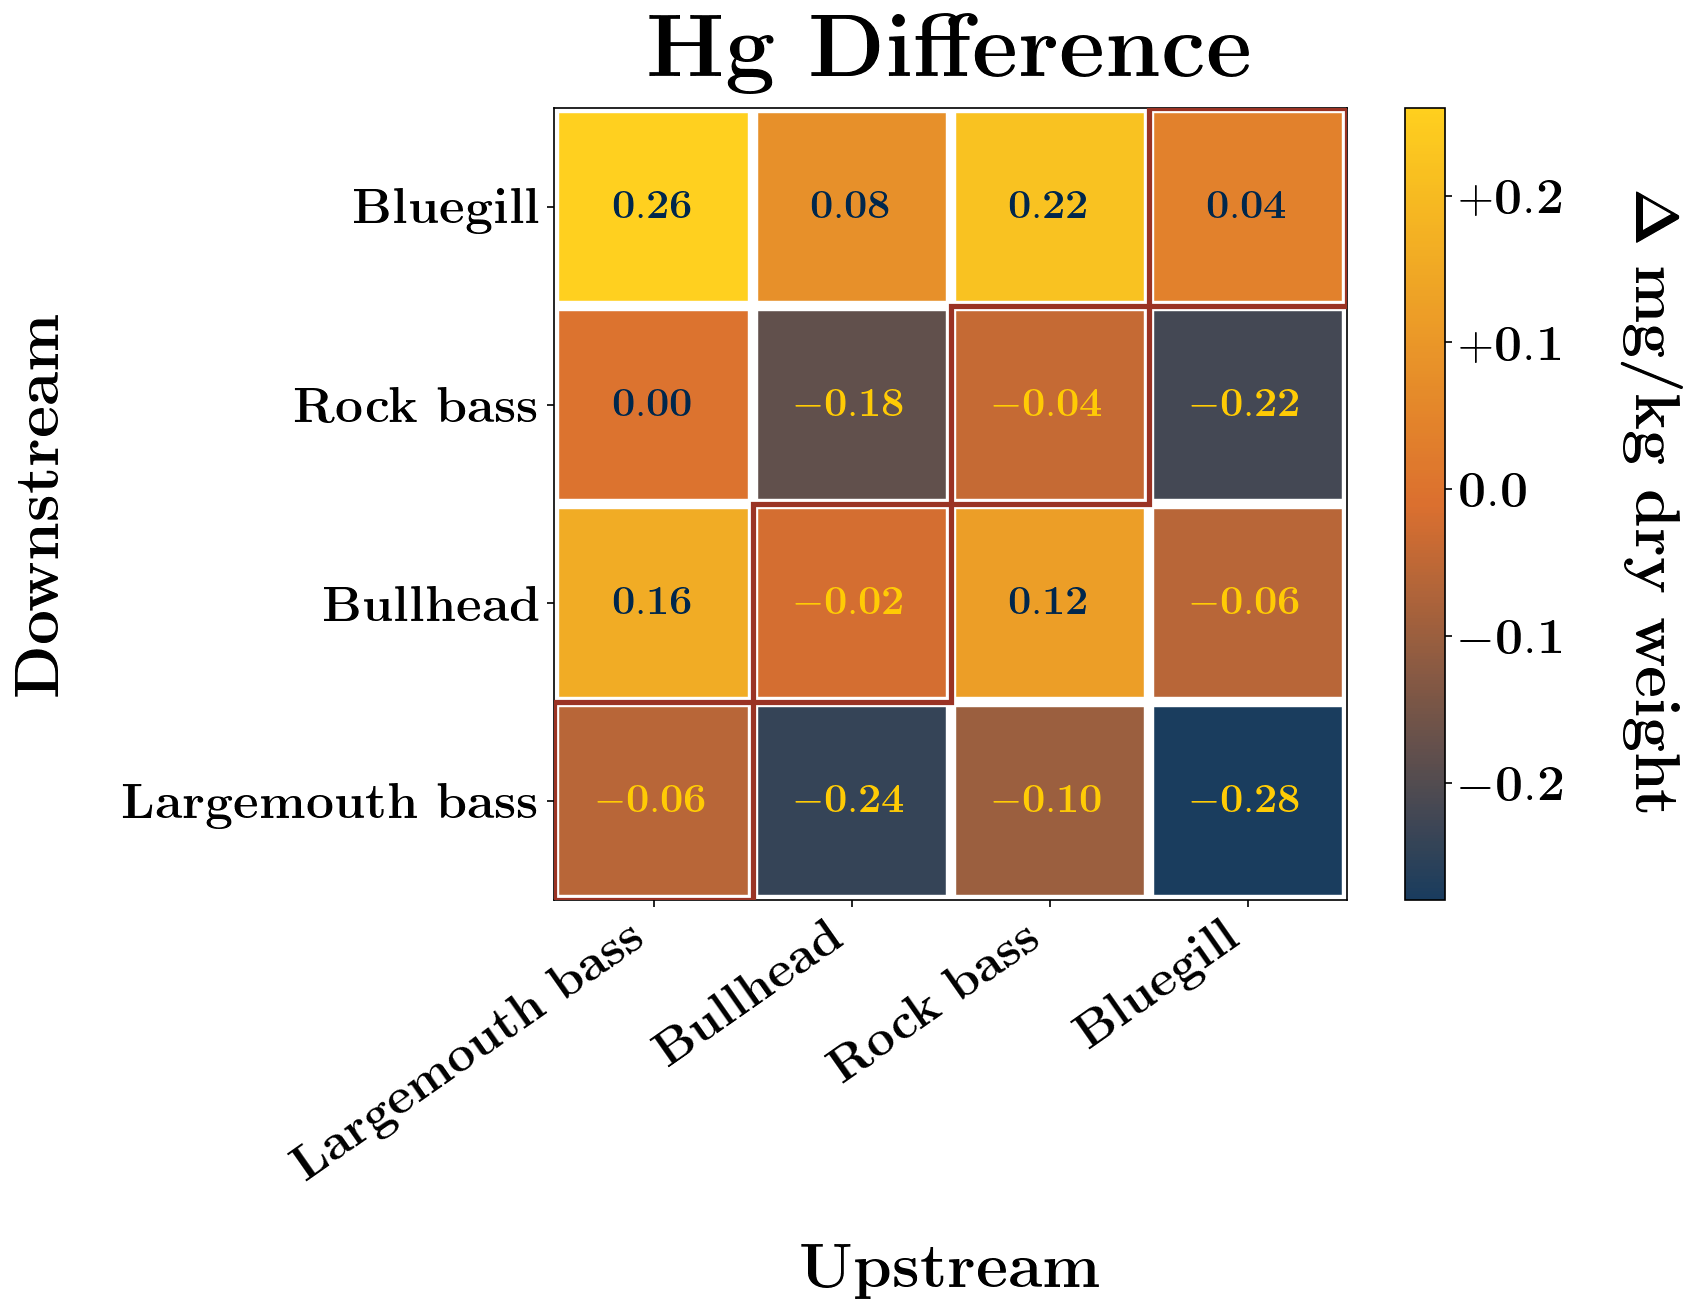
\includegraphics[width=0.99\textwidth]{Img/Hg.png} \\

  \end{center}
  {\small
  Figure 4. Mercury levels were compared between the same species captured below the dam and above the  dam. 
  The values represent the difference in mg/kg of mercury between species from downstream vs upstream $ (downstream - upstream) $.
  }
}
%%%%%%%%%%%%%%%%%%%%%%%%%%%%%%%%%%%%%%%%%%%%%%%%%%%%%%%%%%%%%%%%%%%%%%%%%%%%%%%%%%%%
%%% Benthic Macroinvertebrates %%%%%%%%%%%%%%%%%%%%%%%%%%%%%%%%%%%%%%%%%%%%%%%%%%%%%
%%%%%%%%%%%%%%%%%%%%%%%%%%%%%%%%%%%%%%%%%%%%%%%%%%%%%%%%%%%%%%%%%%%%%%%%%%%%%%%%%%%%
\headerbox{Benthic Macroinvertebrates}{name=box20, column=2, row=0}{
  \begin{center}
    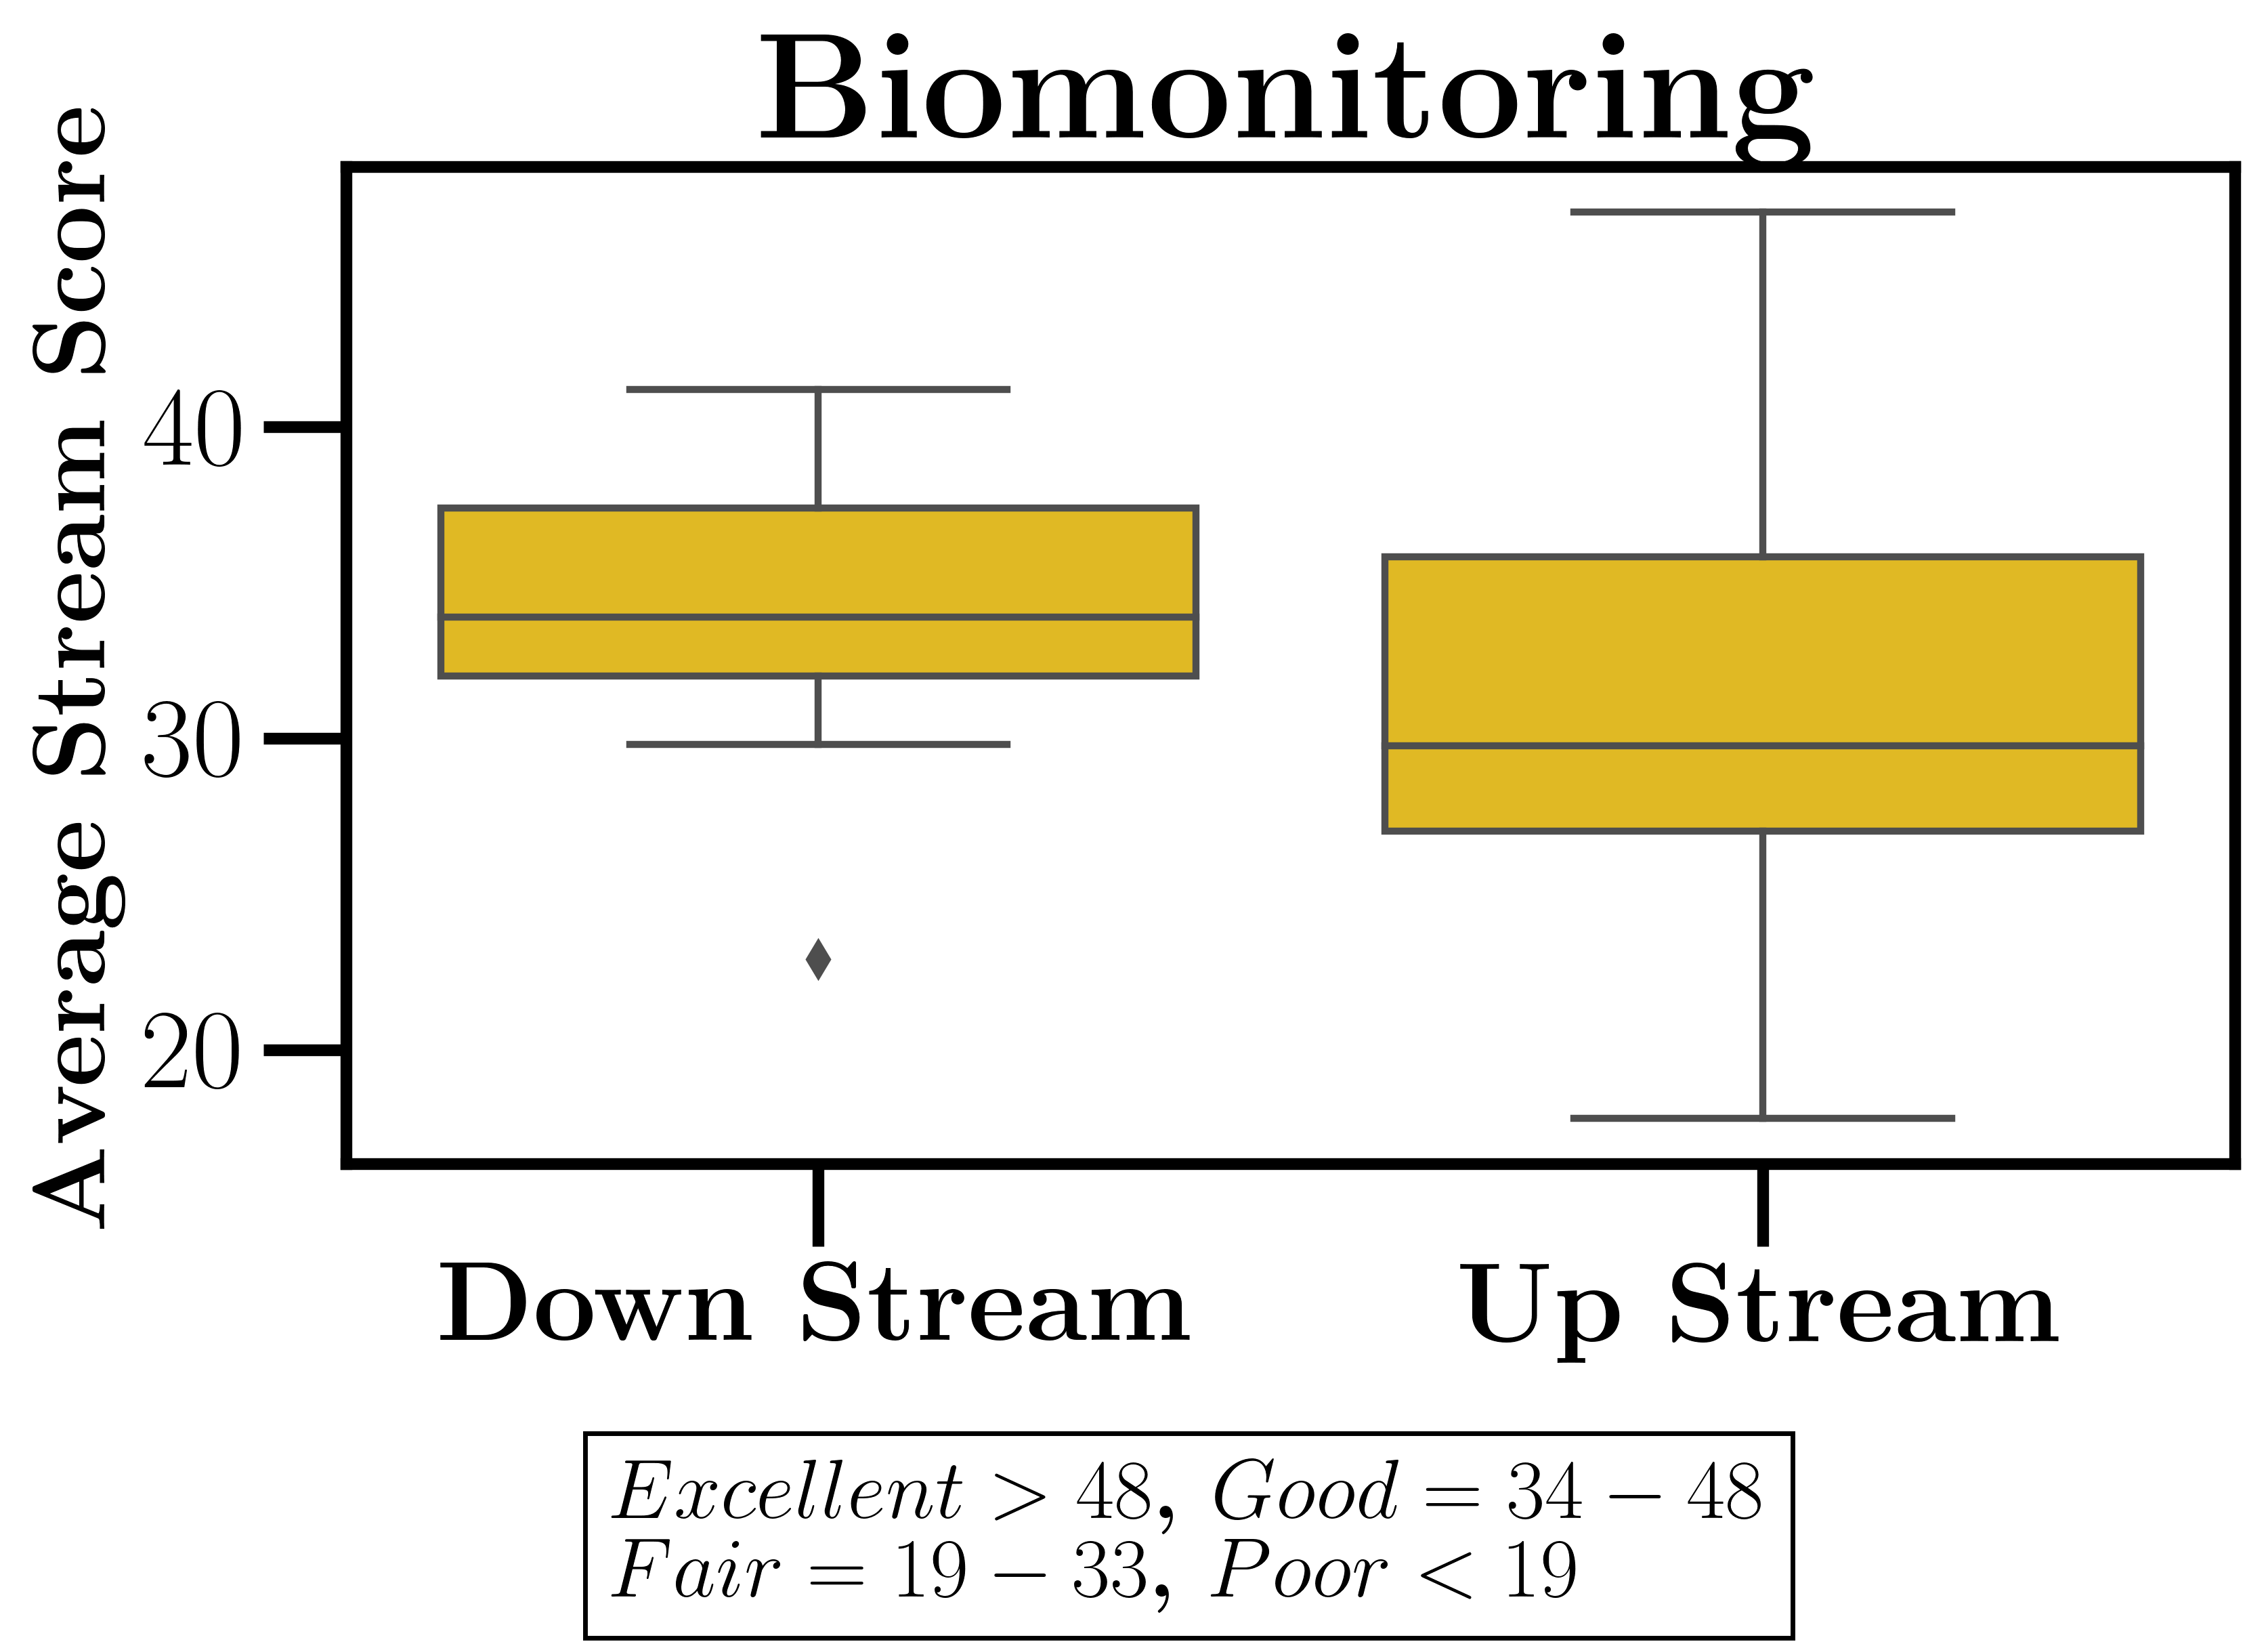
\includegraphics[width=0.99\textwidth]{Img/Biomonitoring.png} \\

  \end{center}
  {\small
  Figure 5. The average stream score assessed through benthic monitoring within the Flint River Watershed. 
  Data was collected from above and below the Hamilton Dam.
  }
}
%%%%%%%%%%%%%%%%%%%%%%%%%%%%%%%%%%%%%%%%%%%%%%%%%%%%%%%%%%%%%%%%%%%%%%%%%%%%%%%%%%%%
%%% Fish Diversity %%%%%%%%%%%%%%%%%%%%%%%%%%%%%%%%%%%%%%%%%%%%%%%%%%%%%%%%%%%%%%%%%
%%%%%%%%%%%%%%%%%%%%%%%%%%%%%%%%%%%%%%%%%%%%%%%%%%%%%%%%%%%%%%%%%%%%%%%%%%%%%%%%%%%%
\headerbox{Fish Diversity}{name=box21, column=2, row=1, below=box20}{
  \begin{center}
    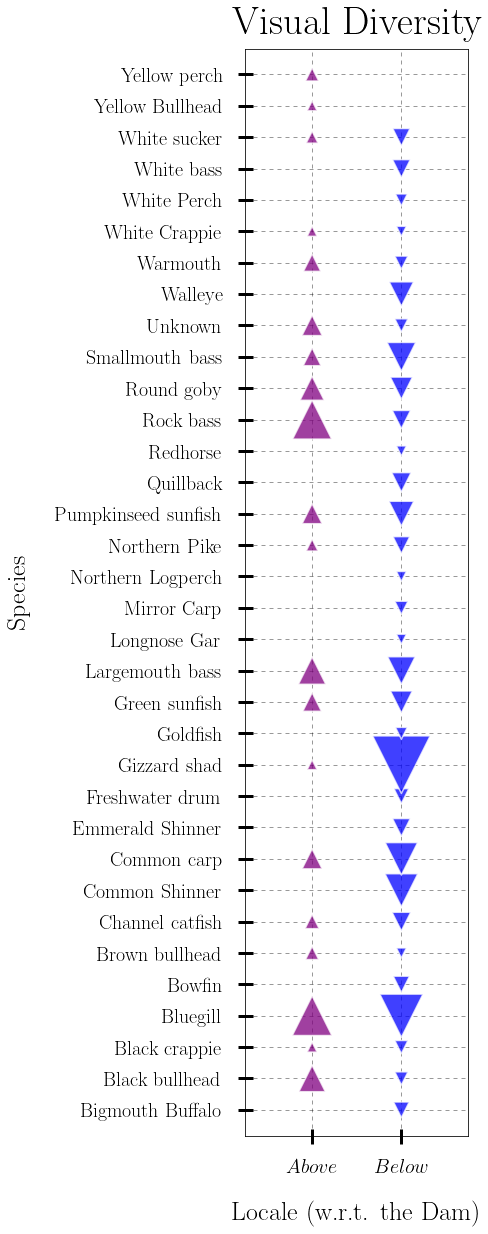
\includegraphics[width=0.93\textwidth]{Img/Diversity_Bubble_Plot.png} \\

  \end{center}
  {\small
  Figure 6. Catches are compared between \\ downstream sites and upstream sites. 
  Notable differences show much higher catches of gizzard shad below the dam and rock bass above the dam.
  }
}
%%%%%%%%%%%%%%%%%%%%%%%%%%%%%%%%%%%%%%%%%%%%%%%%%%%%%%%%%%%%%%%%%%%%%%%%%%%%%%%%%%%%
%%% Discussion %%%%%%%%%%%%%%%%%%%%%%%%%%%%%%%%%%%%%%%%%%%%%%%%%%%%%%%%%%%%%%%%%%%%%
%%%%%%%%%%%%%%%%%%%%%%%%%%%%%%%%%%%%%%%%%%%%%%%%%%%%%%%%%%%%%%%%%%%%%%%%%%%%%%%%%%%%
\headerbox{Discussion}{name=box30, column=3, row=0}{
  \textbf{Hypothesis 1 was supported only in \\ non-piscivorous fish.}
  \begin{itemize}[leftmargin=11.5pt] \small
    \item Mercury levels were higher in  paired species caught downstream vs 
    upstream except in \\ piscivorous fish (Figure 4).
    \item There were more species downstream with higher levels of mercury likely due 
    to the fact that Great Lakes–influenced fish bring more contaminants downstream.
  \end{itemize} 
  \textbf{Hypothesis 2 was supported.}
  \begin{itemize}[leftmargin=11.5pt] \small
    \item Water quality scores based on benthic macroinvertebrates were ``good'' upstream, 
    and downstream we found a lot of zebra \\ mussels rather than benthic \\ macroinvertebrates (Figure 5).
    \item Water quality scores based on benthic macroinvertebrates in the 
    City of Flint are lower where channelization of the river is \\ common.
  \end{itemize}
  \textbf{Hypothesis 3 was not supported.}
  \begin{itemize}[leftmargin=11.5pt] \small
    \item Using Simpson’s diversity index fish diversity was found to be lower 
    downstream, 0.67, than upstream, 0.75.
    \item Even though 31 species were caught downstream vs. 20 upstream, 
    the overall catch was dominated by Gizzard shad downstream, 
    making the species evenness and thus the diversity less than upstream (Figure 6).
  \end{itemize}
}
%%%%%%%%%%%%%%%%%%%%%%%%%%%%%%%%%%%%%%%%%%%%%%%%%%%%%%%%%%%%%%%%%%%%%%%%%%%%%%%%%%%%
%%% Acknowledgements %%%%%%%%%%%%%%%%%%%%%%%%%%%%%%%%%%%%%%%%%%%%%%%%%%%%%%%%%%%%%%%
%%%%%%%%%%%%%%%%%%%%%%%%%%%%%%%%%%%%%%%%%%%%%%%%%%%%%%%%%%%%%%%%%%%%%%%%%%%%%%%%%%%%
\headerbox{Acknowledgements}{name=box31, column=3, row=1, below=box30}{
  {\footnotesize
    \centerline{For funding and support we thank \dots}
    \begin{itemize}[leftmargin=11.5pt]
      \item The Community Foundation of Greater Flint.
      \item Saginaw Bay Watershed Initiative Network.
      \item UM-Flint Office of Research.
      \item UM-Flint CAS Opportunity Fund.
      \item UM-Flint Urban Institute for Racial, Economic, \\ \& Enviornmental Justice.
      \item The Gary and Colleen Pace Field Biology Scholarship.
      \item Those who have worked on or helped with the project including Megan Heyza and many UM-Flint students.
      \item The Flint River Watershed Coalition.
    \end{itemize}
  }
}
%%%%%%%%%%%%%%%%%%%%%%%%%%%%%%%%%%%%%%%%%%%%%%%%%%%%%%%%%%%%%%%%%%%%%%%%%%%%%%%%%%%%
%%% References %%%%%%%%%%%%%%%%%%%%%%%%%%%%%%%%%%%%%%%%%%%%%%%%%%%%%%%%%%%%%%%%%%%%%
%%%%%%%%%%%%%%%%%%%%%%%%%%%%%%%%%%%%%%%%%%%%%%%%%%%%%%%%%%%%%%%%%%%%%%%%%%%%%%%%%%%%
\headerbox{References}{name=box32, column=3, row=2, above=bottom, below=box31}{
  {\footnotesize
    \textbf{[1]} Bankston, N. (2014). 
    Automobile Industry Growth from 1916 to 1989: The Effect on Flint, Michigan Climate. \vspace{0.75mm} \\ 
    \textbf{[2]} Bernier, J., Brousseau, P., Krzystyniak, K., Tryphonas, H., \& Fournier, M. (1995). 
    Immunotoxicity of heavy metals in relation to Great Lakes. 
    Environmental health perspectives, 103 Suppl 9, 23-34. \vspace{0.75mm} \\ 
    \textbf{[3]} McGoldrick, D. J., \& Murphy, E. W. (2016). 
    \\ Concentration and distribution of contaminants in lake trout and walleye from the Laurentian Great Lakes (2008–2012). 
    Environmental Pollution, 217, 85-96. \vspace{0.75mm} \\ 
  }
}

\end{poster}
\end{document}
